\section{Predictive map theory} \label{sec: predictive map theory}
To explain the principle of the predictive map theory introduced in~\cite{StBoGe17HPM}, it is necessary to illustrate the concept of a \cognitiveroom{}, mentioned before in \secreff{sec: Hippocampus}. An example is of course a naive navigational task as presented by \etal{Stachenfeld} and similar to the setting of \figref{\ref{fig: Rat in maze}}. The authors even demonstrated that just a topological environment is sufficient to craft a \cognitiveroom{} and apply the predictive map theory.

The concept becomes far more interesting when talking about cognitive rooms founded on experience \ie the speed of vehicles based on weight and engine specifications. This category of a \cognitiveroom{} also fits the topic of the thesis much better, since it aims to model language not a spatial environment. An illustrating example can be found in \figref{\ref{fig: vehicles cognitive room}}. For instance, a ``sports car'' might be rather lightweight but has plenty of horse power.
\begin{figure}
	\centering
		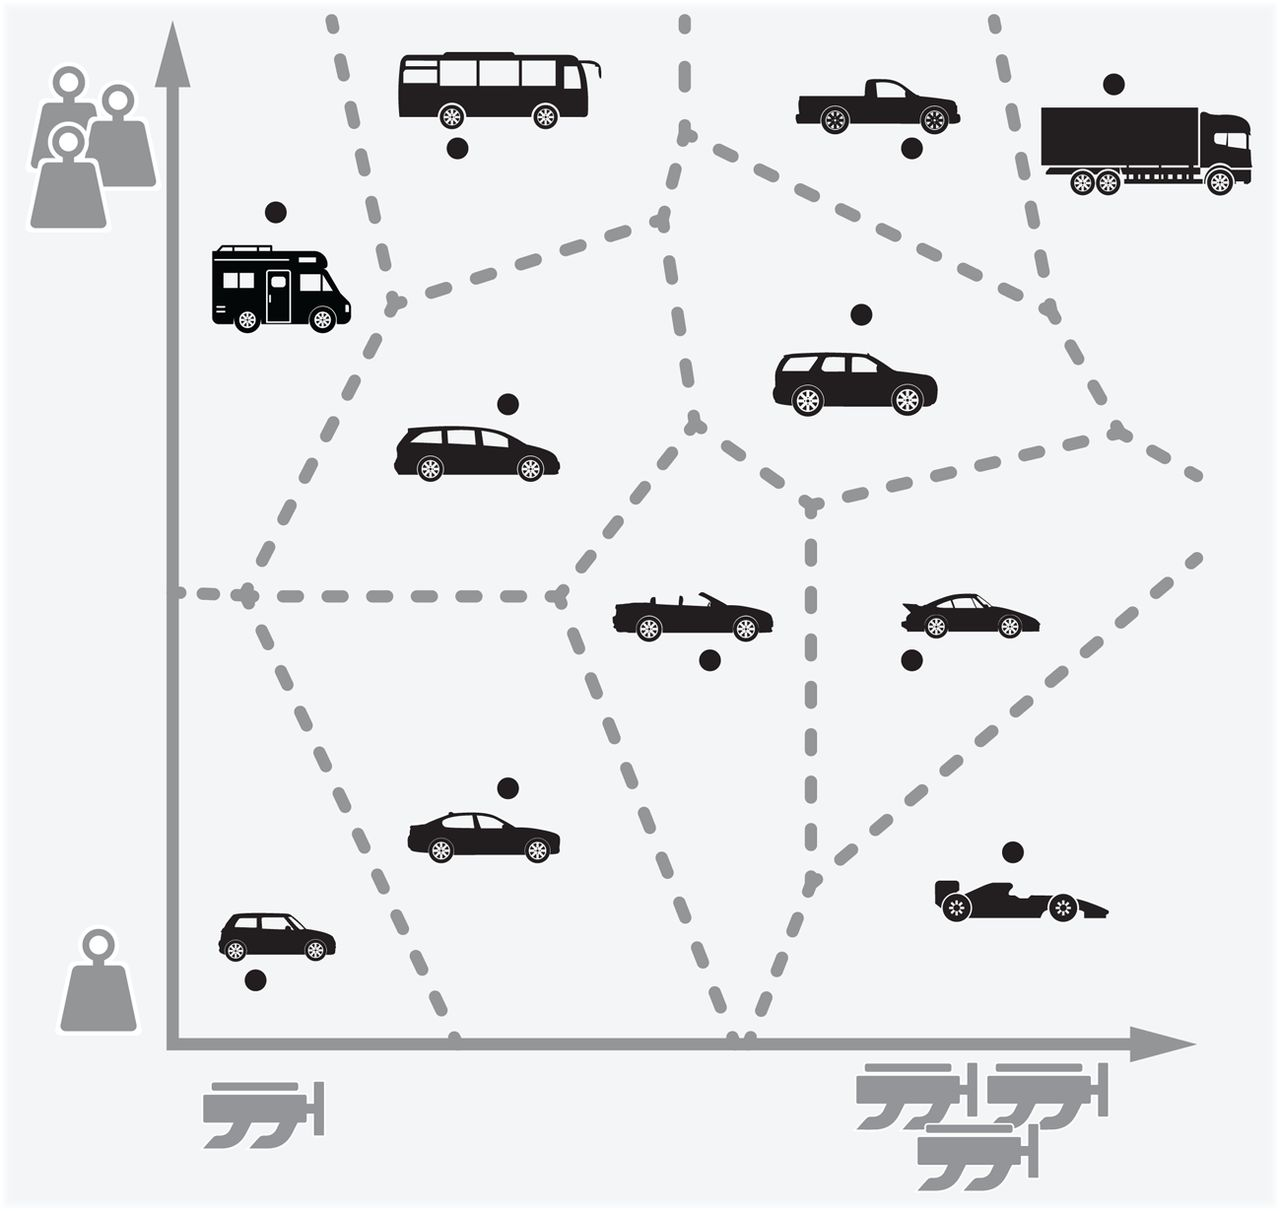
\includegraphics[width=0.4\textwidth]{Fahrzeuge_Cognitive_Room.jpeg}
	\caption{Exemplary \cognitiveroom{} of vehicles according to their weight and engine power. An unknown car can be placed easily in the environment given the two parameters because there are already established place cells acting as abstract waypoints (the depicted cars) to support the orientation \ie finding its place on the map. By doing so, it is immediately possible to derive information about the appearance of the automobile~\cite{BellmundEtAl18NC}.}
	\label{fig: vehicles cognitive room}
\end{figure}
By using these two characteristics, the \cognitiveroom{} has the shape of a $ 2d $-plane. For instance, while reading about an alien car, it is immediately possible to compare it with different well-known vehicles and draw conclusions about its shape since the \cognitiveroom{} has enough information to position the car within it. All these decisions of placing new objects in an appropriate context is done by place and grid cells (\secreff{sec: Hippocampus}). Expanding the example by the firing of cells results in the full illustration given in \figref{\ref{fig: vehicles with place and grid cells}}.
\begin{figure}
	\centering
		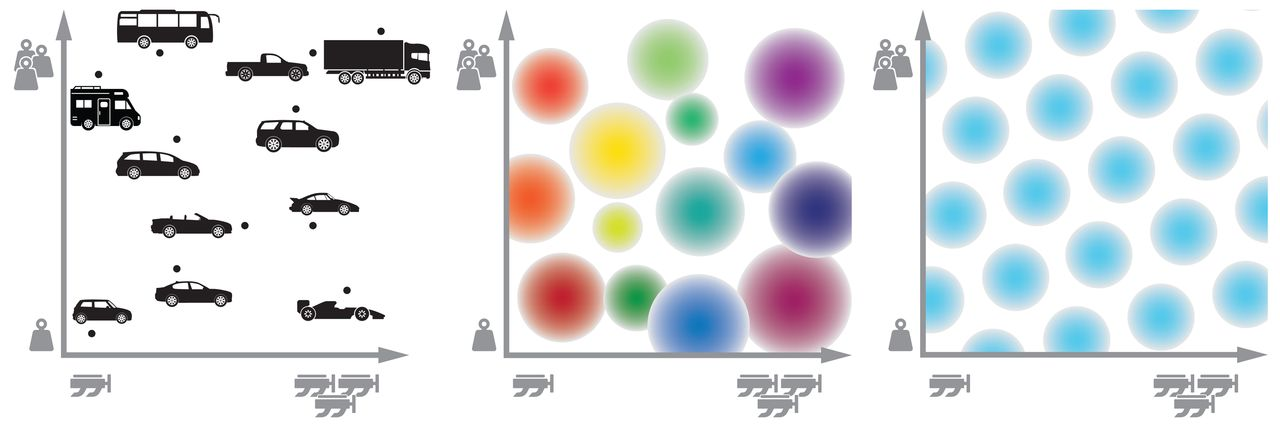
\includegraphics[width=1.\textwidth]{Fahrzeuge_Ortszelle_Gitterzelle.jpeg}
	\caption{Left: \cognitiveroom{} of vehicles according to weight and horse power. Middle: Firing pattern of place cells crafting the \cognitiveroom{} \ie the boundaries in \figref{\ref{fig: vehicles cognitive room}}. Right: Corresponding lattice of grid cells.~\cite{BellmundEtAl18NC}}
	\label{fig: vehicles with place and grid cells}
\end{figure}

%
% Paul bezieht die „Prdictive Map theory“ lediglich „auf die Autos und Tiere“
%

%In case of encountering a unknown species the predictive map becomes active in terms of firing place cells encoding animals sharing the same features and thus evaluating the potential danger. In these terms a place cell doesn't encode the current state but a future state because the new living being will be cataloged next to the known ones. So, the cognitive room exhibits a predictive property.
%
%We can, for instance, apply it to the scenario of the rat passing a maze as seen in Fig. \ref{fig: Rat in maze}. In par. \nameref{par: Place cell} was mentioned that a place cell resembles the current position. By the new perspective follows that the cell fires beforehand~\eg again in terms of the turquoise cell: This cell is now contemplated active if the rat is within the are preceding the arch and aims to enter it.
%
%Furthermore, the authors argue that
